\documentclass[11pt,a4paper]{article}

% ------------------------------------------------------------
% Q-Charge: Product, System Architecture, Optimization and
% Deployment Specification
% Compile on Overleaf with pdfLaTeX.
% ------------------------------------------------------------

\usepackage[a4paper,margin=0.85in]{geometry}
\usepackage[T1]{fontenc}
\usepackage[utf8]{inputenc}
\usepackage{lmodern}
\usepackage{microtype}
\usepackage{xcolor}
\usepackage{graphicx}
\usepackage{booktabs}
\usepackage{tabularx}
\usepackage{longtable}
\usepackage{array}
\usepackage{enumitem}
\usepackage{amsmath,amssymb}
\usepackage{hyperref}
\usepackage{xurl}
\usepackage{tikz}
\usepackage{float}
\usepackage{fancyhdr}
\usepackage{titlesec}
\usepackage{listings}
\usetikzlibrary{arrows.meta,positioning,shapes.geometric,fit,calc}

\definecolor{qgreen}{HTML}{43B581}
\definecolor{qnavy}{HTML}{152238}
\definecolor{qorange}{HTML}{F28C28}
\definecolor{qgray}{HTML}{F3F5F7}
\definecolor{qblue}{HTML}{2878B5}

\hypersetup{
  colorlinks=true,
  linkcolor=qblue,
  urlcolor=qblue,
  citecolor=qblue,
  pdftitle={Q-Charge: Quantum-Assisted EV Charging Optimization Platform},
  pdfsubject={Product and technical specification}
}

\setlength{\parskip}{5pt}
\setlength{\parindent}{0pt}
\setlist[itemize]{leftmargin=1.4em,itemsep=2pt,topsep=3pt}
\setlist[enumerate]{leftmargin=1.6em,itemsep=3pt,topsep=3pt}
\renewcommand{\arraystretch}{1.2}
\pagestyle{fancy}
\fancyhf{}
\lhead{\textcolor{qnavy}{Q-Charge}}
\rhead{\textcolor{qnavy}{Product and Technical Specification}}
\cfoot{\thepage}
\setlength{\headheight}{14pt}

\titleformat{\section}{\Large\bfseries\color{qnavy}}{\thesection}{0.7em}{}
\titleformat{\subsection}{\large\bfseries\color{qnavy}}{\thesubsection}{0.7em}{}
\titleformat{\subsubsection}{\normalsize\bfseries\color{qnavy}}{\thesubsubsection}{0.7em}{}

\lstdefinestyle{code}{
  basicstyle=\ttfamily\small,
  breaklines=true,
  frame=single,
  rulecolor=\color{qgray},
  backgroundcolor=\color{qgray},
  showstringspaces=false,
  columns=fullflexible
}
\lstset{style=code}

\begin{document}

% ----------------------------- TITLE PAGE -----------------------------
\begin{titlepage}
  \centering
  \vspace*{1.1cm}
  {\Large\bfseries\color{qgreen} Q-CHARGE\par}
  \vspace{0.5cm}
  {\huge\bfseries\color{qnavy} Quantum-Assisted\\[0.15cm] EV Charging Optimization Platform\par}
  \vspace{0.7cm}
  {\large Product Vision, Software Requirements, System Architecture,\\
  Optimization Methodology, Deployment Plan and Related Research\par}
  \vspace{1.1cm}
  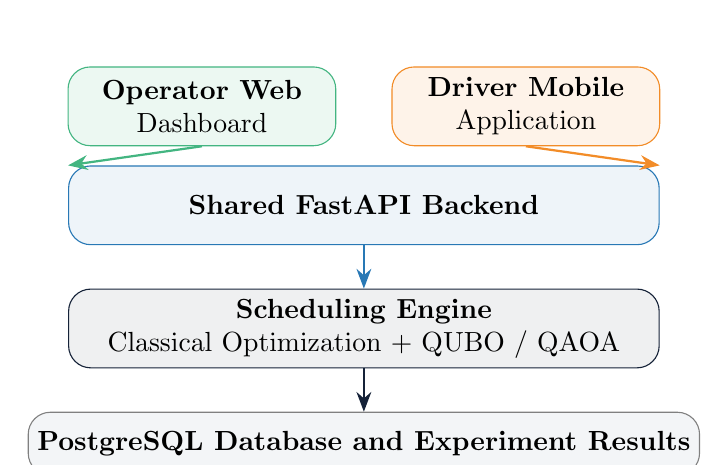
\begin{tikzpicture}[node distance=0.45cm]
    \node[draw=qgreen,fill=qgreen!10,rounded corners=8pt,minimum width=3.4cm,minimum height=1.0cm,align=center] (web) {\textbf{Operator Web}\\Dashboard};
    \node[draw=qorange,fill=qorange!10,rounded corners=8pt,minimum width=3.4cm,minimum height=1.0cm,align=center,right=0.7cm of web] (mobile) {\textbf{Driver Mobile}\\Application};
    \node[draw=qblue,fill=qblue!8,rounded corners=8pt,minimum width=7.5cm,minimum height=1.0cm,align=center,below=0.75cm of $(web)!0.5!(mobile)$] (api) {\textbf{Shared FastAPI Backend}};
    \node[draw=qnavy,fill=qnavy!7,rounded corners=8pt,minimum width=7.5cm,minimum height=1.0cm,align=center,below=0.55cm of api] (opt) {\textbf{Scheduling Engine}\\Classical Optimization + QUBO / QAOA};
    \node[draw=gray,fill=qgray,rounded corners=8pt,minimum width=7.5cm,minimum height=0.8cm,align=center,below=0.55cm of opt] (db) {\textbf{PostgreSQL Database and Experiment Results}};
    \draw[-{Stealth[length=2.5mm]},thick,qgreen] (web.south) -- (api.north west);
    \draw[-{Stealth[length=2.5mm]},thick,qorange] (mobile.south) -- (api.north east);
    \draw[-{Stealth[length=2.5mm]},thick,qblue] (api) -- (opt);
    \draw[-{Stealth[length=2.5mm]},thick,qnavy] (opt) -- (db);
  \end{tikzpicture}
  \vfill
  {\large Technical planning document\par}
  \vspace{0.3cm}
  {\small Version 1.0 \quad|\quad \today\par}
\end{titlepage}

\tableofcontents
\newpage

% ----------------------------- EXECUTIVE SUMMARY -----------------------------
\section{Executive Summary}

Q-Charge is a proposed electric-vehicle (EV) charging management platform that coordinates charging across a station while helping drivers meet their battery and departure requirements. It consists of two client applications sharing one backend: an operator web dashboard and an EV-driver mobile app. Its technical core is a scheduling engine that validates charging constraints, computes a classical baseline, and investigates a quantum-assisted formulation using Quadratic Unconstrained Binary Optimization (QUBO) and the Quantum Approximate Optimization Algorithm (QAOA).

The system is designed to balance electricity cost, station peak demand, charger utilization and driver energy requirements. The first implementation should use simulated stations and synthetic data; real charger hardware and Open Charge Point Protocol (OCPP) integration can be added later. The quantum component is an experimental optimization pathway, not a claim of quantum advantage. Every quantum-assisted result must be checked for feasibility and compared with a classical method on the same instances.

The proposed product stack is React with Vite and TypeScript for the web dashboard, React Native with Expo for mobile, FastAPI for backend services, PostgreSQL for persistent storage, and Python-based optimization components using OR-Tools or SciPy alongside Qiskit. The system can be deployed as separate frontend, API, database and worker services.

\section{Problem Definition}

\subsection{Background}

As EV adoption grows, multiple vehicles may request charging at the same station during overlapping periods. If charging is unmanaged, the station can create high simultaneous power demand, incur avoidable electricity costs under time-varying tariffs, or fail to satisfy drivers' requested battery levels before departure. Scheduling is difficult because vehicles have different arrival times, departure deadlines, battery capacities, current states of charge, target states of charge and charging-rate limits.

\subsection{Problem Statement}

Design and implement a software platform that assigns feasible charging power to EVs over discrete time slots while respecting charger availability and station power limits. The platform should minimize a configurable combination of energy cost and peak demand, while meeting each vehicle's energy requirement when feasible. It should expose the resulting schedule to operators and drivers and provide a reproducible comparison between classical and quantum-assisted optimization.

\subsection{Project Goals}

\begin{itemize}
  \item Generate feasible charging schedules for multiple EVs at a shared station.
  \item Reduce charging cost by shifting flexible demand to lower-price periods.
  \item Limit peak station demand without violating hard electrical constraints.
  \item Help drivers understand their recommended charging windows and estimated costs.
  \item Compare classical and QAOA-based approaches using the same test instances.
  \item Provide an extensible architecture for future renewable-energy forecasts, multiple stations and hardware integration.
\end{itemize}

\subsection{Scope and Non-Goals}

\textbf{Included in the initial product:} simulated stations, configurable EV requests, time-slot scheduling, cost and peak metrics, classical optimization, a small QUBO/QAOA experiment, operator analytics, driver schedule views and deployment-ready APIs.

\textbf{Not assumed in the initial release:} direct control of real chargers, payment processing, guaranteed real-time availability of physical chargers, utility-grade grid control, or demonstrated quantum advantage. These require additional integrations, testing and operational safeguards.

\section{Users and Product Experience}

\subsection{Operator Web Dashboard}

The operator dashboard is the control center for a station or a fleet of stations. Its main capabilities are:
\begin{itemize}
  \item Station overview: number of EVs, charger status, aggregate demand and alerts.
  \item EV queue: arrival, departure, current and target state of charge, and charging power limits.
  \item Infrastructure configuration: charger count, charger power, station power limit and tariffs.
  \item Schedule generation: create or rerun a schedule using selected optimization methods.
  \item Schedule visualization: show each EV's assigned charging periods on a timeline.
  \item Solver comparison: compare feasibility, energy cost, peak load, utilization and runtime.
  \item Reporting: export scenario inputs and evaluation results for research and demonstration.
\end{itemize}

\subsection{EV-Driver Mobile Application}

The driver application exposes the same schedule service through a simpler, driver-focused experience:
\begin{itemize}
  \item Create a vehicle profile with battery capacity and maximum charging rate.
  \item Submit current battery level, desired target level, arrival time and departure deadline.
  \item Select or view a compatible station.
  \item Receive the recommended charging window, charger assignment and estimated cost.
  \item View schedule status and any changes made by the operator.
  \item Optionally receive reminders and notifications in a later release.
\end{itemize}

The driver app should not independently calculate schedules. It should submit requests to the shared backend and display the validated result returned by the scheduling engine.

\subsection{Shared Product Principle}

The web dashboard and mobile app are separate user interfaces, not separate systems. Authentication, vehicle data, station data, scheduling logic, optimization jobs and results must be managed centrally by the backend. This avoids duplicated business rules and keeps the driver-visible schedule consistent with the operator's schedule.

\section{Functional Requirements}

\begin{longtable}{p{1.2cm}p{4.0cm}p{8.0cm}}
\toprule
\textbf{ID} & \textbf{Requirement} & \textbf{Description} \\
\midrule
FR-01 & Vehicle request management & Create and update EV requests including arrival, departure, battery capacity, current SoC, target SoC and maximum charging power. \\
FR-02 & Station configuration & Configure charger count, charger power limits, station power capacity and electricity tariff by time slot. \\
FR-03 & Feasibility validation & Reject invalid requests and detect cases where a target cannot be met within the available window. \\
FR-04 & Classical scheduling & Generate a feasible baseline schedule using a classical solver or heuristic. \\
FR-05 & Quantum-assisted scheduling & Convert a small, bounded scheduling instance into a QUBO and run QAOA through a simulator or supported quantum execution provider. \\
FR-06 & Schedule validation & Independently verify charger, power, timing and energy constraints before returning any schedule as feasible. \\
FR-07 & Metrics & Compute energy cost, peak demand, energy delivered, target completion rate, charger utilization and solver runtime. \\
FR-08 & Operator dashboard & Display station status, EV requests, schedules and comparison metrics. \\
FR-09 & Driver schedule view & Display the driver's assigned charging window, target level and estimated cost. \\
FR-10 & Experiment history & Persist scenario inputs, solver settings, outputs and evaluation metrics for reproducibility. \\
FR-11 & Authentication and roles & Separate driver and operator permissions. \\
FR-12 & Export & Allow authorized users to export schedule and benchmark results. \\
\bottomrule
\end{longtable}

\section{Non-Functional Requirements}

\begin{itemize}
  \item \textbf{Correctness:} every schedule labelled feasible must pass an independent constraint validator.
  \item \textbf{Reliability:} solver errors, timeouts and infeasible scenarios must return clear status messages.
  \item \textbf{Security:} use HTTPS, validated inputs, secure password/session handling, role-based access and protected secrets.
  \item \textbf{Privacy:} collect only the driver data required for scheduling; use synthetic or anonymized data in demonstrations.
  \item \textbf{Maintainability:} separate API routes, domain services, optimizer implementations and database models.
  \item \textbf{Reproducibility:} record scenario parameters, random seeds where applicable, solver versions and run duration.
  \item \textbf{Scalability:} allow expensive optimization jobs to move from the API process to a separate worker.
  \item \textbf{Usability:} the operator can run a scenario and interpret the schedule and metrics without reading raw solver output.
\end{itemize}

\section{System Architecture}

\subsection{Logical Architecture}

\begin{figure}[H]
\centering
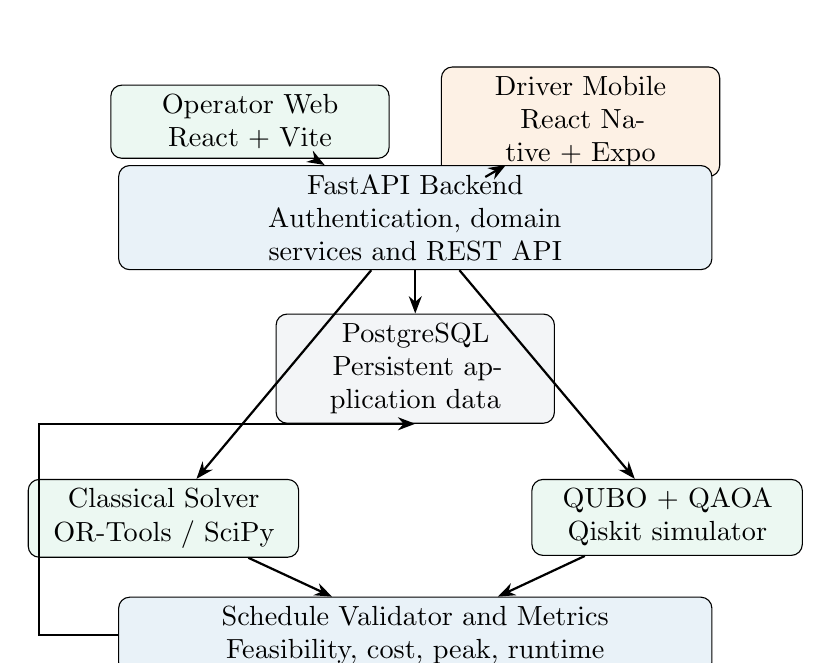
\begin{tikzpicture}[
  node distance=0.55cm and 0.65cm,
  box/.style={draw,rounded corners=4pt,align=center,minimum height=0.8cm,text width=3.3cm,fill=qgray},
  api/.style={box,fill=qblue!10,text width=7.3cm},
  opt/.style={box,fill=qgreen!10,text width=3.2cm},
  arr/.style={-{Stealth[length=2.2mm]},thick}
]
\node[box,fill=qgreen!10] (web) {Operator Web\\React + Vite};
\node[box,fill=qorange!12,right=of web] (mobile) {Driver Mobile\\React Native + Expo};
\node[api,below=of $(web)!0.5!(mobile)$] (api) {FastAPI Backend\\Authentication, domain services and REST API};
\node[box,below=of api] (db) {PostgreSQL\\Persistent application data};
\node[opt,below left=0.7cm and -0.3cm of db] (classical) {Classical Solver\\OR-Tools / SciPy};
\node[opt,below right=0.7cm and -0.3cm of db] (quantum) {QUBO + QAOA\\Qiskit simulator};
\node[api,below=1.0cm of $(classical)!0.5!(quantum)$] (validate) {Schedule Validator and Metrics\\Feasibility, cost, peak, runtime};
\draw[arr] (web) -- (api);
\draw[arr] (mobile) -- (api);
\draw[arr] (api) -- (db);
\draw[arr] (api) -- (classical);
\draw[arr] (api) -- (quantum);
\draw[arr] (classical) -- (validate);
\draw[arr] (quantum) -- (validate);
\draw[arr] (validate.west) -- ++(-1.0,0) |- (db.south);
\end{tikzpicture}
\caption{Q-Charge logical architecture. The API coordinates the solvers; all returned schedules pass through a common validator.}
\end{figure}

\subsection{Suggested Repository Structure}

\begin{lstlisting}
q-charge/
  apps/
    operator-web/       # React + Vite + TypeScript
    driver-mobile/      # React Native + Expo
  services/
    api/                # FastAPI routes and domain services
    optimizer/          # classical and QAOA implementations
    worker/             # optional background job worker
  packages/
    shared-types/       # API types and validation contracts
  migrations/           # Alembic migrations
  tests/
    unit/
    integration/
    optimization/
  docker-compose.yml
  README.md
\end{lstlisting}

The exact folder layout can be adjusted to match the repository tooling, but frontend code, backend code and optimization logic should remain clearly separated.

\subsection{Technology Stack}

\begin{tabularx}{\textwidth}{p{3.1cm}X}
\toprule
\textbf{Layer} & \textbf{Recommended technology} \\
\midrule
Operator frontend & React, Vite, TypeScript, Tailwind CSS \\
Driver mobile app & React Native, Expo, TypeScript \\
Charts & Recharts or an equivalent React chart library \\
Backend API & Python, FastAPI, Pydantic \\
Database & PostgreSQL \\
ORM and migrations & SQLAlchemy and Alembic \\
Classical optimization & OR-Tools or SciPy; use a solver appropriate to the final formulation \\
Quantum optimization & Qiskit and QAOA; start with small instances on a simulator \\
Data and analysis & NumPy, Pandas, Matplotlib \\
Testing & Pytest, frontend component tests and API integration tests \\
Deployment & Docker, managed web hosting, API hosting and managed PostgreSQL \\
Version control & Git and GitHub \\
\bottomrule
\end{tabularx}

\section{Data Model}

The following entities are a starting schema. They can be normalized further during implementation.

\begin{longtable}{p{3.0cm}p{9.9cm}}
\toprule
\textbf{Entity} & \textbf{Key fields and purpose} \\
\midrule
User & id, email, password hash or identity-provider id, role, created\_at. Supports driver/operator permissions. \\
Vehicle & id, owner\_id, battery\_capacity\_kwh, max\_charging\_kw, connector\_type, optional vehicle metadata. \\
Station & id, name, location, max\_grid\_power\_kw, tariff configuration, station status. \\
Charger & id, station\_id, max\_power\_kw, connector type, status. \\
ChargingRequest & id, vehicle\_id, station\_id, arrival time, departure deadline, current SoC, target SoC, request status. \\
OptimizationJob & id, station\_id, method, parameters, status, created\_at, started\_at, completed\_at, error summary. \\
Schedule & id, optimization\_job\_id, request\_id, charger\_id, time slot, assigned power, energy delivered. \\
ExperimentResult & id, optimization\_job\_id, feasibility, total cost, peak power, completion rate, utilization, runtime, solver metadata. \\
\bottomrule
\end{longtable}

Store timestamps consistently, preferably in UTC in the database, and convert to the station's local time zone for display. Define the meaning of each time slot clearly (for example, 15-minute intervals) and use the same convention in all solvers.

\section{API Design}

Use a versioned REST API under \texttt{/api/v1}. The table below describes proposed endpoints, not an already deployed API.

\begin{longtable}{p{1.4cm}p{5.1cm}p{6.4cm}}
\toprule
\textbf{Method} & \textbf{Endpoint} & \textbf{Purpose} \\
\midrule
GET & \texttt{/health} & Service health check. \\
POST & \texttt{/auth/register} & Create a user account, if local authentication is used. \\
POST & \texttt{/auth/login} & Authenticate a user. \\
GET & \texttt{/stations} & List stations visible to the current user. \\
POST & \texttt{/stations} & Create a station for an authorized operator. \\
GET & \texttt{/stations/\{id\}/chargers} & Retrieve charger configuration and status. \\
POST & \texttt{/charging-requests} & Submit a driver's charging request. \\
GET & \texttt{/charging-requests/\{id\}} & Retrieve request details and status. \\
POST & \texttt{/optimization-jobs} & Start a classical, QAOA or comparison run. \\
GET & \texttt{/optimization-jobs/\{id\}} & Retrieve job status and solver results. \\
GET & \texttt{/optimization-jobs/\{id\}/schedule} & Retrieve the validated schedule. \\
GET & \texttt{/stations/\{id\}/metrics} & Retrieve cost, peak, utilization and completion metrics. \\
\bottomrule
\end{longtable}

For long-running jobs, return a job identifier and status such as \texttt{queued}, \texttt{running}, \texttt{completed}, \texttt{failed} or \texttt{infeasible}. The clients can poll the job endpoint initially; server-sent events or WebSockets can be considered later if live updates are necessary.

\section{Optimization Formulation}

\subsection{Time Discretization and Decision Variables}

Divide the scheduling horizon into slots indexed by \(t \in T\). Let \(i \in V\) represent an EV. A simple binary formulation uses
\[
x_{i,t} =
\begin{cases}
1 & \text{if EV } i \text{ charges in slot } t,\\
0 & \text{otherwise.}
\end{cases}
\]
If charging power can vary, use \(p_{i,t}\) as a continuous power variable in a classical mixed-integer model. A binary fixed-power model is easier to map to QUBO but may be less expressive.

Let \(c_t\) be the electricity price per kWh in slot \(t\), \(\Delta t\) the slot duration in hours, \(P_i^{\max}\) the maximum power for EV \(i\), \(P^{\mathrm{grid}}\) the station power limit, and \(E_i^{\mathrm{need}}\) the energy required by EV \(i\) to reach its target state of charge.

\subsection{Objective Function}

A conceptual objective is
\[
\min \quad
\lambda_c \sum_{t\in T} c_t \Delta t \sum_{i\in V} p_{i,t}
+ \lambda_p P_{\mathrm{peak}}
+ \lambda_u \Phi_{\mathrm{user}},
\]
where \(P_{\mathrm{peak}}\) is the maximum aggregate charging power and \(\Phi_{\mathrm{user}}\) represents any explicitly defined soft penalty for unmet energy demand or preference violations. Hard safety and feasibility constraints must not be replaced solely by soft penalties. The weights \(\lambda_c,\lambda_p,\lambda_u\) should be documented and tested for sensitivity.

\subsection{Core Constraints}

\textbf{Availability:}
\[
p_{i,t}=0 \quad \text{for slots outside EV } i\text{'s arrival--departure window.}
\]

\textbf{Charging rate:}
\[
0 \leq p_{i,t} \leq P_i^{\max}.
\]

\textbf{Station power limit:}
\[
\sum_{i\in V} p_{i,t} \leq P^{\mathrm{grid}}
\quad \forall t\in T.
\]

\textbf{Energy requirement:}
\[
\sum_{t\in T} \eta_i p_{i,t}\Delta t
\geq E_i^{\mathrm{need}}
\]
for every request whose target is feasible, where \(\eta_i\) represents the modeled charging efficiency. In the implementation, use a consistent battery-energy convention and avoid double-counting efficiency.

\textbf{Charger availability:} the schedule must not assign more simultaneous sessions than the number of compatible available chargers. If each charger serves at most one EV in a slot, this can be expressed with assignment variables \(y_{i,j,t}\) and charger-specific constraints.

\textbf{Departure deadline:} energy required for a request must be delivered before its departure deadline. If the request is physically infeasible, return an explicit infeasible status or the best-effort result clearly labelled as such.

\subsection{Classical Baseline}

Implement and test a transparent baseline before attempting QAOA. Useful baselines include:
\begin{itemize}
  \item First-Come, First-Served (FCFS), as a simple operational reference.
  \item A classical optimization model using OR-Tools or SciPy, selected to match the variable types and constraints.
  \item Optionally, a heuristic such as earliest-deadline-first for additional comparisons.
\end{itemize}

The exact classical model should be capable of producing a validated schedule and reporting infeasibility when the constraints cannot be met. A classical solver is not merely a fallback; it is the reference needed to evaluate the quantum experiment.

\subsection{QUBO and QAOA Pathway}

QUBO represents a problem using binary variables \(z\) and a quadratic objective:
\[
\min_{z\in\{0,1\}^n} \quad z^\top Qz.
\]
Constraints can be encoded using penalty terms, for example:
\[
E_{\mathrm{QUBO}}(z) =
E_{\mathrm{cost}}(z)
+ A E_{\mathrm{capacity}}(z)
+ B E_{\mathrm{energy}}(z)
+ C E_{\mathrm{assignment}}(z),
\]
where \(A,B,C\) are penalty weights. The mapping must be designed carefully: poor penalty weights can cause infeasible solutions to score better than feasible ones, and binary encodings can grow rapidly with the number of EVs and time slots.

QAOA uses a parameterized quantum circuit to sample candidate binary solutions. In Q-Charge, the first experiments should use small, controlled instances that can be independently checked by exhaustive enumeration or a trusted classical solver. QAOA outputs must pass through the same schedule validator as classical outputs. Report circuit size, number of variables, depth \(p\), shot count, optimization settings, simulator or hardware backend, runtime, best objective and feasibility rate.

\textbf{Important research limitation:} QAOA is a quantum optimization method; it is not itself a quantum machine-learning model. If a competition track specifically requires QML, confirm that quantum optimization is eligible or add a justified learning component as a separate module. Do not claim quantum advantage unless the evaluation provides evidence for it.

\section{Evaluation Plan}

\subsection{Metrics}

\begin{tabularx}{\textwidth}{p{3.2cm}X}
\toprule
\textbf{Metric} & \textbf{Definition / purpose} \\
\midrule
Feasibility rate & Percentage of runs producing schedules that satisfy all hard constraints. \\
Energy cost & Sum of delivered energy multiplied by the applicable time-slot price. \\
Peak demand & Maximum aggregate charging power across the scheduling horizon. \\
Target completion rate & Fraction of EV requests meeting their target energy before departure. \\
Charger utilization & Fraction of available charger-time occupied by charging sessions. \\
Runtime & Wall-clock time to produce and validate a schedule, including solver setup where appropriate. \\
Objective quality & Objective value computed consistently for each valid schedule. \\
Robustness & Results across different seeds, tariffs, arrival patterns and scenario sizes. \\
\bottomrule
\end{tabularx}

\subsection{Experiment Design}

\begin{enumerate}
  \item Create fixed benchmark scenarios with documented EV counts, chargers, time slots, tariffs and power limits.
  \item Use identical inputs and objective definitions for FCFS, the classical solver and QAOA.
  \item Run multiple random seeds where the algorithm is stochastic and record all solver settings.
  \item Validate every candidate schedule independently before computing comparative metrics.
  \item Report infeasible instances separately instead of hiding them or treating them as successful runs.
  \item Compare results by instance size and report limitations, including QAOA circuit size and simulation time.
\end{enumerate}

The evaluation should avoid comparing a strong classical optimizer against an intentionally weak quantum baseline. Include a transparent baseline and, where feasible, an exact solution for small instances to estimate optimality gaps.

\section{Deployment Architecture and Plan}

\subsection{Recommended Hosting Pattern}

\begin{itemize}
  \item \textbf{Web dashboard:} deploy the React/Vite build to a static frontend host such as Vercel.
  \item \textbf{API:} deploy FastAPI as a Python web service on a host such as Render or Railway.
  \item \textbf{Database:} use managed PostgreSQL, for example Neon or a PostgreSQL offering from the API host.
  \item \textbf{Mobile application:} use Expo Application Services (EAS) to build installable Android/iOS artifacts. Public store release is a separate step.
  \item \textbf{Optimizer worker:} run expensive or long-running jobs in a separate worker process/service once needed.
  \item \textbf{Repository and CI:} use GitHub for version control, review and automated test/build workflows.
\end{itemize}

Provider plans, limits and prices can change. Check current documentation before choosing a production plan. The listed providers are architectural options, not endorsements or a guarantee that every plan supports every workload.

\subsection{Deployment Sequence}

\begin{enumerate}
  \item Create the repository and configure development, testing and production environment variables.
  \item Create PostgreSQL and run database migrations.
  \item Deploy the FastAPI backend and verify its health endpoint and API documentation.
  \item Deploy the operator web app and configure its public API base URL.
  \item Run an end-to-end test: submit a request, run a solver, validate the schedule and display the result.
  \item Configure the Expo application with the deployed API URL and build an installable test app.
  \item Move heavy optimization jobs to a worker if API latency or hosting limits require it.
  \item Configure logs, monitoring, backups, access controls and a repeatable deployment pipeline.
\end{enumerate}

\subsection{Environment Variables}

Example names only; actual secret values must be stored in the hosting provider's secret manager and must never be committed to version control.

\begin{lstlisting}
# Backend
DATABASE_URL=postgresql://...
SECRET_KEY=<generated-secret>
CORS_ORIGINS=https://your-dashboard-domain.example

# Web frontend (public value only)
VITE_API_URL=https://your-api-domain.example

# Mobile application
EXPO_PUBLIC_API_URL=https://your-api-domain.example
\end{lstlisting}

Variables exposed to browser or mobile bundles are not secret. Database credentials, signing keys and private tokens must remain on the server side. Restrict CORS to known origins, enforce authorization in the API, and use HTTPS in deployed environments.

\subsection{Operational Considerations}

A local SQLite database is suitable for early development, but a persistent managed database is preferable for a deployed multi-user service. Hosted filesystems may be ephemeral. Long-running QAOA experiments should not block ordinary API requests; create a job record and let a worker execute the optimization, then store the result for clients to retrieve.

\section{Security, Privacy and Reliability}

\begin{itemize}
  \item Enforce role-based authorization for operator-only station management and driver-owned requests.
  \item Hash passwords using a modern password-hashing library if local authentication is used; never store plain-text passwords.
  \item Validate all inputs server-side, including time ranges, battery percentages, power limits and station identifiers.
  \item Use parameterized database access through the ORM and maintain database migrations.
  \item Keep credentials out of source control and rotate exposed secrets.
  \item Avoid exposing detailed exception traces to users; retain structured server logs without unnecessary personal information.
  \item Back up the database and test recovery procedures before a public production release.
  \item Label simulated charger status and estimated costs clearly; do not present simulated telemetry as real physical measurements.
  \item Ensure the optimizer cannot send commands to physical chargers unless a separate, authorized hardware-control layer has been designed and safety-tested.
\end{itemize}

\section{Implementation Roadmap}

\begin{longtable}{p{1.3cm}p{3.2cm}p{8.5cm}}
\toprule
\textbf{Phase} & \textbf{Workstream} & \textbf{Deliverables} \\
\midrule
1 & Requirements and setup & User journeys, architecture decision record, repository structure, development environment and issue backlog. \\
2 & Simulator and data model & EV/station/charger models, synthetic scenarios, time-slot convention and input validation. \\
3 & Classical optimizer & FCFS baseline, constrained classical solver, independent validator and unit tests. \\
4 & Quantum experiment & Small QUBO formulation, QAOA implementation, documented penalty weights and reproducible experiments. \\
5 & Backend API & Authentication, station/request endpoints, optimization jobs, result storage and OpenAPI documentation. \\
6 & Operator dashboard & Station overview, EV queue, schedule timeline, solver comparison and metrics. \\
7 & Driver app & Vehicle profile, charging request form, recommended schedule and status display. \\
8 & Integration and hardening & End-to-end tests, error states, authorization, migrations, logs and backups. \\
9 & Deployment and evaluation & Hosted demo, Android test build, benchmark report, documentation and presentation walkthrough. \\
\bottomrule
\end{longtable}

\section{Testing Strategy}

\subsection{Unit Tests}
Test SoC-to-energy calculations, charging efficiency, tariff calculations, time-slot boundaries, charger compatibility and constraint validation.

\subsection{Optimization Tests}
Use small scenarios whose optimal solution can be verified by enumeration. Test impossible deadlines, insufficient station power, overlapping requests, no available chargers, zero-energy requests and varying tariffs. Confirm that invalid schedules are never marked feasible.

\subsection{API and Integration Tests}
Test authentication, role permissions, request validation, database persistence, job lifecycle, solver failure handling and consistency between the schedule returned to the operator and the schedule shown to the driver.

\subsection{Frontend and Mobile Tests}
Test loading, success, empty, invalid and error states. Verify that displayed metrics are obtained from backend results rather than hard-coded demo values. Test the mobile app on a physical device against the deployed API.

\section{Related Open-Source Projects}

The following projects are useful references for learning and design. They are not components that must be copied into Q-Charge. Review each repository's current license, maintenance state and attribution requirements before reusing code.

\begin{longtable}{p{3.2cm}p{5.4cm}p{4.3cm}}
\toprule
\textbf{Project} & \textbf{Relevance} & \textbf{Link} \\
\midrule
SAP eMobility Smart Charging & EV fleet charging schedules, infrastructure constraints, cost and peak-load objectives, REST API. Implemented in Java/Spring Boot. & \url{https://github.com/SAP/emobility-smart-charging} \\
QAOA Knapsack EV Charging & Direct quantum-optimization reference for a constrained EV charging allocation problem. & \url{https://github.com/QCL-PKNU/QAOA-Knapsack-EV-Charging} \\
ACN Portal / ACN-Sim & Research tools, EV charging simulation, charging-session data access and algorithm comparison. & \url{https://github.com/zach401/acnportal} \\
SteVe & Open-source OCPP server and charging-station management concepts. Useful for future hardware integration. & \url{https://github.com/steve-community/steve} \\
Qiskit Optimization & Quantum optimization modeling and algorithm examples. Check current project status and IBM's recommended successor tooling before adopting. & \url{https://github.com/qiskit-community/qiskit-optimization} \\
\bottomrule
\end{longtable}

\section{Related Research Papers}

The papers below provide background for the optimization problem and quantum formulation. Read the methods and limitations, not only the abstract. The first paper is the most directly related QAOA charging reference; the review provides broader context.

\begin{enumerate}[label={[R\arabic*]}]
  \item K. Kea, C. Huot, and Y. Han, ``Leveraging Knapsack QAOA Approach for Optimal Electric Vehicle Charging,'' \textit{IEEE Access}, vol. 11, pp. 109964--109973, 2023. DOI: \href{https://doi.org/10.1109/ACCESS.2023.3320800}{10.1109/ACCESS.2023.3320800}. Official code: \url{https://github.com/QCL-PKNU/QAOA-Knapsack-EV-Charging}. A correction was published in 2025; check it when reviewing the results.
  \item C. Si, K. T. Chau, W. Liu, and Y. Hou, ``Optimal scheduling for electric vehicle charging: A review of methods, technologies, and uncertainty management,'' \textit{Journal of Energy Storage}, 2025, article 117500. DOI: \href{https://doi.org/10.1016/j.est.2025.117500}{10.1016/j.est.2025.117500}.
  \item A. Okada, K. Otaki, and H. Yoshida, ``Joint optimization of electric vehicle routes and charging locations through learning charge constraints using QUBO solvers,'' \textit{Scientific Reports}, vol. 16, article 25090, 2026. DOI: \href{https://doi.org/10.1038/s41598-026-55392-1}{10.1038/s41598-026-55392-1}. This concerns routing and station placement rather than exactly the same station scheduling problem.
  \item P. and S. K. Sood, ``Cost-efficient energy utilization of idle electric vehicles through quantum-optimized vehicle-to-vehicle charging,'' \textit{Journal of Energy Storage}, 2026, article 122534. DOI: \href{https://doi.org/10.1016/j.est.2026.122534}{10.1016/j.est.2026.122534}. This is a related extension involving vehicle-to-vehicle charging, not the core Q-Charge use case.
\end{enumerate}

\subsection{How the References Inform Q-Charge}

\begin{itemize}
  \item Use SAP Smart Charging to understand a practical charging optimizer and its API-oriented architecture.
  \item Use the QAOA knapsack paper and its code to study quantum encoding, penalties and experiments.
  \item Use ACN-Sim to learn how charging algorithms can be evaluated in repeatable scenarios.
  \item Use SteVe to understand OCPP and station-management concepts if real charger integration becomes a goal.
  \item Use the review paper to map classical optimization, uncertainty and operational challenges before claiming a research gap.
\end{itemize}

\textbf{Research positioning:} combining EV scheduling with QAOA is not automatically novel. A defensible contribution should be based on a specific, measured question—for example, how feasibility and solution quality change with instance size, how penalty weights affect constraint satisfaction, or how a hybrid solver performs against strong classical baselines under the same objective and test scenarios.

\section{Risks and Mitigations}

\begin{longtable}{p{3.4cm}p{5.1cm}p{4.4cm}}
\toprule
\textbf{Risk} & \textbf{Impact} & \textbf{Mitigation} \\
\midrule
QUBO size grows quickly & QAOA circuits and simulation become impractical as variables increase. & Start with small instances, document encoding size and use classical solvers for larger cases. \\
Penalty weights are poorly tuned & The optimizer may prefer an infeasible schedule. & Run penalty sensitivity tests and independently validate every schedule. \\
No quantum advantage is observed & Quantum results may be slower or lower quality than classical results. & Report honestly; treat the project as a comparative study, not a guaranteed speedup. \\
Infeasible driver request & Target SoC cannot be reached by departure. & Detect infeasibility early and communicate the reason and best-effort alternatives. \\
API and worker timeouts & Long optimization runs can interrupt requests. & Use job records, timeouts, retries where safe and a separate worker. \\
Provider limits or cost changes & Hosting may not support a workload or plan as expected. & Check current limits, measure resource use and keep deployment configuration portable. \\
Hardware integration complexity & Real chargers require protocols, authentication and safety checks. & Begin with simulation; treat OCPP and physical control as a separate, tested integration. \\
\bottomrule
\end{longtable}

\section{Success Criteria}

Q-Charge should be considered ready for a credible demonstration when:
\begin{itemize}
  \item A driver can submit a valid charging request through the mobile app.
  \item The shared backend stores the request and starts an optimization job.
  \item The classical solver returns a schedule or a clear infeasibility result.
  \item The QAOA experiment runs on a documented small instance and its result is independently validated.
  \item The operator dashboard compares solver results using the same scenario and metrics.
  \item The driver app displays the schedule stored by the backend rather than calculating a separate one.
  \item The deployed application handles failures, invalid input and authorization checks without exposing secrets.
  \item The report presents reproducible measurements and does not claim unsupported quantum advantage.
\end{itemize}

\section{Conclusion}

Q-Charge is conceived as a shared-backend EV charging product with two complementary applications: an operator web dashboard and a driver mobile app. Its central engineering challenge is to produce safe, feasible and explainable charging schedules. Its research component is to investigate whether a carefully formulated QUBO/QAOA approach offers useful behavior on specific small EV scheduling instances compared with strong classical baselines.

The recommended path is to formalize the data model and constraints, implement the simulator and classical baseline, build and validate a small quantum experiment, then connect the web and mobile clients to the same backend. Deployment, benchmarking and transparent documentation should be treated as part of the product rather than as final cosmetic tasks.

\end{document}
